\chapter{ServletContext和Web配置}
\label{chp:JavaEE-ServletContext-and-Web-configuration}

\section*{基本信息}
\sline
\begin{description}
\item[课程名称:] Java应用与开发
\item[授课教师:] 王晓东
\item[授课时间:] 第十一周
\item[参考教材:] 本课程参考教材及资料如下:
  \begin{itemize}
  \item 吕海东,张坤 编著,Java EE企业级应用开发实例教程,清华大学出版社,2010年8月
  \end{itemize}
\end{description}

\section*{教学目标}

\sline

{\hei\Blue Java EE Web应用需要部署在符合Java EE规范的Web容器中运行,
  如何取得Web应用本身的信息在编程中非常重要。}

\begin{enumerate}
\item 掌握Web应用对象ServletContext。
\item 了解Web应用的配置方法。
\item 掌握MVC模式Web开发中发挥核心作用的转发,区别{\hei 转发}与{\hei 重定向}。
\end{enumerate}  

\section*{授课方式}

\sline
\begin{description}
\item[理论课:] 多媒体教学、程序演示
\item[实验课:] 上机编程
\end{description}

\newpage
\section*{教学内容}
\sline

%%%%%%%%%%%%%%%%%%%%%%%%%%%%%%%%%%%%%%%%%%%%%%%%%%%%%%%%%%%%%%
\section{Web应用环境对象}

\subsection{Web应用环境对象} 

将Web应用部署到服务器上,启动Web服务器后,Web容器为每个Web应用创建一个
表达Web应用环境的对象(即ServletContext对象),并将Web应用的基本信息存
储在这个ServletContext对象中。

\tta{Web应用环境对象的用途} 

\begin{itemize}\kai
\item 所有Web组件都可以访问此ServletContext对象,进而取得Web应用的基本
  信息。
\item ServletContext还可以作为整个Web应用的共享容器对象,能够被所有会话
  请求共用,保存Web应用的共享信息。
\end{itemize}


\subsection{Web应用环境对象的生命周期} 

ServletContext对象的生命周期与Web应用相同。

\begin{description}
\item[创建] Web容器启动后,自动创建ServletContext对象;
\item[销毁] Web容器停止时,自动销毁ServletContext对象。
\end{description}

  
\notice{注意}

{\kai 如果在ServletContext对象中保存的对象信息需要长久保存,一般编
  写ServletContext对象的监听器,在此对象销毁之前将其中保存的对象数据进
  行持久化处理,如保存到数据库或者文件中。}

\subsection{Web应用环境对象的类型和取得} 

Web应用环境对象是接口{\bf\Blue javax.servlet.ServletContext}的实现。

\tta{在Servlet内直接取得ServletContext接口对象}

\begin{javaCode}
  ServletContext ctx = this.getServletContext();
\end{javaCode}


\subsection{Web应用环境对象的功能和方法} 

\tta{Web级数据共享容器}

\ttc{public void setAttribute(String name, Object object)}

对象保存到ServletContext。

\begin{javaCode}
  ServletContext ctx = this.getServletContext();
  ctx.setAttribute("userId", "Kevin");
  ctx.setAttribute("age", 20); //自动完成 int 类型转换为 Integer 对象类型
\end{javaCode}

\ttc{public Object getAttribute(String name)}

读取保存在ServletContext对象中指定名称的属性对象,不存在则返回null。

\begin{javaCode}
  String useId = (String) ctx.getAttribute("userId");
  int age = (Integer) ctx.getAttribute("age"); //自动拆箱,将 Integer 转为 int
\end{javaCode}


\ttc{public void removeAttribute(String name)}

将指定的属性从ServletContext对象中删除。

\ttc{Enumeration getAttributeNames()}

取得所有属性的名称列表,返回一个枚举器对象,可以用于遍历所有属性名称。
\begin{javaCode}
  Enumeration nums = ctx.getAttributeName();
  while (nums.hasMoreElements()) {
    System.out.println(nums.nextElements());
  }
\end{javaCode}

\notice{注意} ServletContext大量的方法请自行学习掌握。

%%%%\begin{frame}[fragile] % [fragile]参数使得能够插入代码
%%%%  \subsection{Web应用环境对象的功能和方法} 
%%%%
%%%%  \wxd{读取Web级初始化参数}
%%%%
%%%%  一般不要在代码中放置各种外部资源的连接参数,如数据库驱动、连接URL等,否则会导致参数更改时需要重新编译Java代码。
%%%%
%%%%  一般的做法是将这些参数放置在Web配置文件/WEB-INF/web.xml中,提高了系统的可维护性。(后续讲解)
%%%%
%%%%  \wxd{访问外部资源}
%%%%
%%%%  ServletContext对象提供了访问外部资源的方法:
%%%%  
%%%%  \begin{itemize}
%%%%  \item 取得Web文档的绝对路径
%%%%  \item 配合I/O流读写Web文档
%%%%  \item 取得转发对象
%%%%  \item 实现服务器端Web组件的转发
%%%%  \end{itemize}
%%%%\end{frame}
%%%%\begin{frame}[fragile] % [fragile]参数使得能够插入代码
%%%%  \subsection{Web应用环境对象的功能和方法} 
%%%%
%%%%  \xyy{public String getRealPath(String path)}
%%%%
%%%%  取得指定Web目录或文档的绝对目录地址,Path要求以“/”开头,表示Web根目录。如,取得Web目录/upload的绝对目录地址,当使用文件上传功能组件时此方法有用。
%%%%
%%%%  \begin{javaCode}
%%%%    String realPath = ctx.getRealPath("/upload");
%%%%  \end{javaCode}
%%%%
%%%%  \xyy{public InputStream getResourceAsStream(String path)}
%%%%
%%%%  以二进制字节流的类型返回指定的Web资源,可以是Web应用中的任何文档,包括JSP、图片、声音或视频文件,然后使用Input流读取此文件。
%%%%  \begin{javaCode}
%%%%    InputStream in = ctx.getResourceAsStream("/test.txt");
%%%%
%%%%    int read = in.read();
%%%%    while (read != -1) {
%%%%      System.out.println((char)read);
%%%%      read = in.read();
%%%%    }  
%%%%  \end{javaCode}
%%%%\end{frame}
%%%%
%%%%\begin{frame}[fragile] % [fragile]参数使得能够插入代码
%%%%  \subsection{Web应用环境对象的功能和方法} 
%%%%
%%%%  \xyy{public RequestDispatcher getRequestDispatcher(String path)}
%%%%
%%%%  取得Web文档的转发对象,目的是实现到目标文档的服务器转发。
%%%%
%%%%  \begin{javaCode}
%%%%    try {
%%%%      Thread.sleep(2000);
%%%%    } catch (InterruptedException e) {
%%%%      e.printStackTrace();
%%%%    }
%%%%    RequestDispatcher rd = ctx.getRequestDispatcher("/test.html");
%%%%    rd.forward(request, response);  
%%%%  \end{javaCode}
%%%%
%%%%  注意:要求转发目标地址必须是以“/”开头,表示Web的根目录,否则抛出java.lang.IllegalArgumentException。
%%%%\end{frame}
%%%%
%%%%\begin{frame}[fragile,fragile,fragile] % [fragile]参数使得能够插入代码
%%%%\subsection{服务器环境对象的功能和方法} 
%%%%
%%%%\xyy{public URL getResource(String path) throws MalformedURLException}
%%%%
%%%%返回指定Web资源的URL地址,例如取得Web页面/main.jsp的URL:
%%%%\begin{javaCode}
%%%%java.net.URL url = ctx.getResource("/test.html");
%%%%System.out.println(url.toString());  
%%%%\end{javaCode}
%%%%
%%%%输出结果为:
%%%%\begin{verbatim}
%%%%jndi:/localhost/TestWebProj/test.html
%%%%\end{verbatim}
%%%%
%%%%\xyy{public String getMimeType(String file)}
%%%%
%%%%\begin{javaCode}
%%%%String mime = ctx.getMimeType("/test.html");
%%%%System.out.println(mime);  
%%%%\end{javaCode}
%%%%
%%%%输出结果为:
%%%%
%%%%\begin{verbatim}
%%%%text/html
%%%%\end{verbatim}
%%%%\end{frame}
%%%%
%%%%\begin{frame}[fragile] % [fragile]参数使得能够插入代码
%%%%\subsection{服务器环境对象的功能和方法} 
%%%%
%%%%\wxd{取得Web应用的基本信息}
%%%%
%%%%\xyy{public int getMajorVersion()}
%%%%
%%%%取得Servlet容器的API主版本号。
%%%%
%%%%\xyy{public int getMinorVersion()}
%%%%
%%%%取得Servlet容器的API次版本号。上述两个方法用于测试代码的兼容性。
%%%%
%%%%\xyy{public String getServerInfo()}
%%%%
%%%%取得Web容器的名称和版本信息,即Web服务器的名称和版本。
%%%%
%%%%例如输出:Apache Tomcat/7.0.32
%%%%\end{frame}
%%%%
%%%%\begin{frame}[fragile] % [fragile]参数使得能够插入代码
%%%%\subsection{服务器环境对象的功能和方法} 
%%%%
%%%%\wxd{Web应用日志输出}
%%%%
%%%%项目开发人员为追踪代码的运行情况,尤其是出现异常时的错误信息,经常将此类信息写入日志文件,便于日后监控和维护。
%%%%
%%%%尤其时已经发布运行的项目,不方便到用户现场服务器的控制台进行查看。
%%%%
%%%%一般的做法是配置Web服务器的日志文件到可以远程访问的FTP服务器上,开发人员可以定期从FTP下载日志文件进行分析,找出系统的异常和错误时间和地点。
%%%%
%%%%\xyy{public void log(String msg)}
%%%%
%%%%将指定的消息文本写入到日志文件中。一般用于比较关键的事件,如用户登录应用系统和执行关键的操作像删除产品等。
%%%%\end{frame}
%%%%
%%%%\begin{frame}[fragile] % [fragile]参数使得能够插入代码
%%%%\subsection{服务器环境对象的功能和方法} 
%%%%
%%%%\begin{javaCode}
%%%%String id = request.getParameter("userId");
%%%%String password = request.getParameter("password");
%%%%
%%%%IUser user = BusinessFactory.createUser();
%%%%
%%%%if (user.validate(id, password)) {
%%%%  String ip = request.getRemoteAddr();
%%%%  ServletContext ctx = this.getServletContext();
%%%%  String msg = "User Login: " + id + new Date() + "Time, At" + ip;
%%%%  ctx.log(msg);
%%%%}
%%%%\end{javaCode}
%%%%\end{frame}
%%%%
%%%%\begin{frame}[fragile] % [fragile]参数使得能够插入代码
%%%%\subsection{服务器环境对象的功能和方法} 
%%%%
%%%%\xyy{public void log(String message, Throwable throwable)}
%%%%
%%%%将异常类的跟踪堆栈并附加消息文本写入到LOG日志文件中,一般用于异常处理。
%%%%
%%%%\begin{javaCode}
%%%%try {
%%%%
%%%%}  catch(Exception e) {
%%%%  ctx.log("更新库存余额时错误异常", e);
%%%%}
%%%%\end{javaCode}
%%%%\end{frame}

\section{Java EE Web的配置}

\subsection{配置文件web.xml} 

Web的配置文件为{\bf\Red /WEB-INF/web.xml},/WEB-INF目录
是{\bf\Red 被Web服务器保护的目录},客户端浏览器无法直接访问该目录下的任
何文件,Struts、Spring等框架都将配置文件保存在该目录下。

\subsection{web.xml的主要配置项}

\begin{itemize}
\item Servlet声明(Servlet)
\item Servlet映射(Servlet-mapping)    
\item Web级初始参数(context-param)
\item 过滤器(filter)
\item 过滤器映射(filter-mapping)
\item 监听器(listener)
\item 异常跳转页面(error-page)
\item MIME类型映射(mime-mapping)
\item 会话对象超时(session-config)
\item 外部资源声明(resource-ref)
\item 外部标记库描述符文件(taglib)
\end{itemize}

\subsection{Web初始参数配置} 

\tta{Web初始参数配置}

\begin{xmlCode}
  <context-param>
  <description>数据库驱动</description>
  <param-name>driverName</param-name>
  <param-value>sun.jdbc.odbc.jdbcOdbcDriver</param-value>
  </context-param>
\end{xmlCode}

\tta{Web组件取得Web初始参数}

在Servlet中可以通过ServletContext对象取得Web初始参数。

\ttc{public String getInitParameter(String name)} 取得指定名称的Web初始参数。

\begin{javaCode}
  ServletContext ctx = this.getServletContext();
  String driverName = ctx.getInitParameter("driverName");  
\end{javaCode}

%%%%\begin{frame}[fragile] % [fragile]参数使得能够插入代码
%%%%\subsection{Web初始参数配置} 
%%%%
%%%%\xyy{public Enumeration getInitParameterNames()} 取得所有Web初始参数名称列表,以枚举器类型返回。
%%%%
%%%%\begin{javaCode}
%%%%for (Enumeration ee = ctx.getInitParameterNames(); ee.hasMoreElements(); ) {
%%%%  String paramName = (String) ee.nextElement();
%%%%  System.out.println(paramName + "="  + ctx.getInitParameter(paramName));
%%%%}
%%%%\end{javaCode}
%%%%\end{frame}
%%%%
%%%%\begin{frame}[fragile] % [fragile]参数使得能够插入代码
%%%%\subsection{Web应用级异常处理配置} 
%%%%
%%%%通过配置方式处理异常,当Web应用中Web组件JSP或Servlet抛出异常时,Web容器自动在配置文件中查找对应的异常类型,根据配置自动跳转到异常处理页面。
%%%%
%%%%Java EE提供两种错误配置方法:
%%%%\begin{itemize}\kai
%%%%\item 以错误状态码配置的处理方式。
%%%%\item 以异常类型配置的处理方式。
%%%%\end{itemize}
%%%%\end{frame}
%%%%
%%%%\begin{frame}[fragile] % [fragile]参数使得能够插入代码
%%%%\subsection{Web应用级异常处理配置} 
%%%%
%%%%\wxd{以错误状态码配置的处理方式}
%%%%
%%%%当JSP或Servlet的响应状态码与配置的状态码一致时,Web容器自动跳转到配置的页面。
%%%%
%%%%\begin{xmlCode}
%%%%<error-page>  
%%%%  <error-code>500</error-code>
%%%%  <location>/error/info500.jsp</location>
%%%%</error-page>  
%%%%\end{xmlCode}
%%%%
%%%%如在Servlet中编写如下代码:
%%%%
%%%%\begin{javaCode}
%%%%out.print(10/0); // 会抛出零除异常
%%%%\end{javaCode}
%%%%
%%%%Servlet响应为500,表示内部错误,Web容器将使用配置的/error/info500.jsp页面代替默认的500错误页面。
%%%%\end{frame}
%%%%
%%%%\begin{frame}[fragile] % [fragile]参数使得能够插入代码
%%%%\subsection{Web应用级异常处理配置} 
%%%%
%%%%\wxd{以异常类型配置的处理方式}
%%%%
%%%%\begin{xmlCode}
%%%%<error-page>  
%%%%  <exception-type>java.lang.NullException</exception-type>
%%%%  <location>/error/info500.jsp</location>
%%%%</error-page>  
%%%%\end{xmlCode}
%%%%
%%%%当JSP或Servlet内出现空指针异常时,Web容器将检测到异常,自动转发到所配置的location元素指定的页面。
%%%%
%%%%\end{frame}
%%%%
%%%%
%%%%\begin{frame}[fragile] % [fragile]参数使得能够插入代码
%%%%\subsection{MIME类型映射配置} 
%%%%
%%%%有的文件没有出现在MIME中,需要开发人员手动进行文件和MIME类型的映射,当Web服务器取得此类文件的扩展名时,使用getContextType就可以取出对应的MIME类型。
%%%%
%%%%映射语法如下:
%%%%
%%%%\begin{xmlCode}
%%%%<mime-mapping>  
%%%%  <extension>jpg</extension>
%%%%  <mime-type>image/jpeg</mime-type>
%%%%</mime-mapping>  
%%%%\end{xmlCode}
%%%%
%%%%取得文件images/tu01.jpg的MIME类型:
%%%%
%%%%\begin{javaCode}
%%%%ServletContext ctx = this.getServletContext();
%%%%String mime = ctx.getMimeType("image/tu01.jpg");
%%%%\end{javaCode}
%%%%
%%%%如果输出MIME类型,将显示image/jpeg。
%%%%\end{frame}

\subsection{会话超时配置} 

\tta{在Java代码中配置HttpSession对象的超时时间}

\begin{javaCode}
  HttpSession session = request.getSession();
  session.setMaxInactiveInterval(15 * 60); // 设置会话超时为15分钟
\end{javaCode}

\tta{在Web配置文件中进行会话超时配置}\footnote{推荐在web.xml中配置会话超时。}

\begin{xmlCode}
  <session-config>
  <session-timeout>900</session-timeout>
  </session-config>
\end{xmlCode}

%%%%\begin{frame}[fragile] % [fragile]参数使得能够插入代码
%%%%\subsection{外部资源的引用配置} 
%%%%
%%%%Web应用的Web组件经常需要各种外部资源和服务,如使用Web服务器配置的数据库连接池、JMS消息服务等。
%%%%
%%%%在web.xml中引入资源或服务的配置方法,以配置JNDI服务为例:
%%%%
%%%%\begin{xmlCode}
%%%%<resource-ref>  
%%%%  <description>DB connection</description>
%%%%  <res-ref-name>java:comp/env/cityoa<res-ref-name>
%%%%  <ref-type>java.sql.DataSource</ref-type>
%%%%  <res-auth>Container</res-auth>
%%%%</resource-ref>  
%%%%\end{xmlCode}
%%%%
%%%%取得此连接池的方法:
%%%%
%%%%\begin{javaCode}
%%%%Context context = new InitialContext(); // 初始化 JNDI 服务对象
%%%%DataSource ds = (DataSource) context.lookup("java:comp/env/cityoa");  // 使用引用名
%%%%Connection cn = ds.getConnection(); // 取得连接池中的一个数据库连接
%%%%\end{javaCode}
%%%%\end{frame}

\section{Servlet配置对象}

\subsection{Servlet配置对象ServletConfig}

\begin{itemize}
\item Java EE为取得Servlet的配置信息,提供一个Servlet配置对象API。
\item 该对象在Servlet初始化阶段由Web容器实例化,并将当前Servlet的配置
  数据写入到此对象,供Servlet读取使用。
\end{itemize}

\subsection{配置对象的类型和取得} 

配置对象类型javax.servlet.ServletConfig是一个接口,具体实现类由容器厂商实现。

ServletConfig对象在Servlet的init方法中取得,由Web容器以参数方式注入到Servlet:

\begin{javaCode}
  private ServletConfig config = null;

  public void init(ServletConfig config) throws ServletException {
    super.init(config);
    this.config = config;
  }
\end{javaCode}

\begin{enumerate}\kai
\item 要取得ServletConfig对象需要重写init方法,并传递ServletConfig参数。然后
  在doGet和doPost方法中即可以使用config对象。
\item 与ServletContext和HttpSession对象不同,Web容器为每个Servlet实例创建一
  个ServletConfig对象,不同Servlet之间无法共享此对象。
\end{enumerate}

\subsection{ServletConfig功能和方法} 

\subsubsection{public String getInitParameter(String name)} 

取得指定的Servlet配置参数。与Web初始参数不同,Servlet初始参数在Servlet声明中定义。

\begin{xmlCode}
  <servlet>  
  <servlet-name>ServletConfigSample</servlet-name>
  <servlet-class>ouc.javaee.ServletConfigSample</servlet-class>
  <init-parm>
  <param-name>url</param-name>
  <param-value>jdbc:oracle:thin:@210.30.108.5:1521:oracle</param-value>
  </init-parm>
  </servlet>  
\end{xmlCode}

\notice{注意} {\kai <init-param>标签要放置在<servlet-name>和<servlet-class>后,否则编译错误。}

\tta{取得配置的Servlet初始参数}

\begin{javaCode}
  String url = config.getInitParameter("url");
\end{javaCode}

\subsubsection{public Enumeration getInitParameterNames()}

取得所有Servlet初始化参数。

\ttc{public String getServletName()}

取得Servlet的名称。

\ttb{public ServletContext getServletContext()}

{\kai ServletConfig对象提供了取得ServletContext对象的方法,与在Servlet内使
  用this.getServletContext()一样,返回ServletContext实例的对象引用。}

\begin{javaCode}
  ServletContext ctx = config.getServletConfig();
\end{javaCode}

\section{转发和重定向}

\subsection{Web跳转方式} 

\subsubsection{重定向(redirect)}

典型的重定向跳转方式如下:

\begin{itemize}
\item 地址栏手工输入新的URL地址;
\item 单击超链接;
\item 提交FORM表单;
\item 使用响应对象response的sendRedirect()方法。
\end{itemize}

{\Blue\hei 重定向跳转方法都是由客户端浏览器来执行的,由此可见重定向增加了网络的访问流量。}

\subsubsection{转发(forward)}

\begin{itemize}
\item 转发是在服务器端进行页面直接跳转的方法。
\item 转发是指Web组件在服务器端直接请求到另外Web组件的方式。
\item 转发在Web容器内部完成,不需要通过客户端浏览器,因此客户端浏览器的地址还停留在初次请求的地址上。
\end{itemize}

{\Blue\hei Web开发中应该尽量使用转发实现Web组件之间的导航。}

\subsection{实现转发} 

\tta{取得转发对象}

转发对象类型为javax.servlet.RequestDispatcher。

\ttc{通过请求对象HttpServletRequest取得}

\begin{javaCode}
  RequestDispatcher rd = request.getRequestDispatcher("main.jsp");
\end{javaCode}

\ttc{使用ServletContext对象的方法取得}

\begin{javaCode}
  RequestDispatcher rd = this.getServletContext().getRequestDispatcher("/main.jsp");
\end{javaCode}

取得转发对象后,调用转发对象的方法forward完成转发。

\begin{javaCode}
  RequestDispatcher rd = request.getRequestDispatcher("main.jsp");
  rd.forward(request, response);
\end{javaCode}

\notice{目标页面main.jsp的目录说明}

\begin{itemize}\small\kai
\item 如果上述代码所在的Servlet被映射到/employee/main.action(一个虚
  拟请求地址),则转发的目标页面main.jsp也需要放到/employee目录下;
\item 如果main.jsp和Servlet映射地址不在同一目录,就需要使用相对路径定
  位,如把main.jsp放在/department/main.jsp,则取得转发对象需要按照如
  下示例代码进行修改:
\end{itemize}

\begin{javaCode}
  RequestDispatcher rd =
  request.getRequestDispatcher("../department/main.jsp");
\end{javaCode}

%%%%\begin{frame}[fragile] % [fragile]参数使得能够插入代码
%%%%  \subsection{实现转发的两种方法的区别}
%%%%
%%%%  \begin{itemize}
%%%%  \item {\hei 从请求对象得到的转发对象要求使用相对路径}
%%%%
%%%%    \begin{javaCode}
%%%%      RequestDispatcher rd = request.getRequestDispatcher("../department/main.jsp");
%%%%      rd.forward(request, response);
%%%%    \end{javaCode}
%%%%
%%%%  \item {\hei 从ServletContext对象取得的转发对象要求使用绝对路径},即以“/”开头,否则会抛出java.lang.IllegalArgumentException异常。
%%%%
%%%%    \begin{javaCode}
%%%%      RequestDispatcher rd = request.getRequestDispatcher("/department/main.jsp");
%%%%      rd.forward(request, response);
%%%%    \end{javaCode}
%%%%  \end{itemize}
%%%%\end{frame}
%%%%
%%%%\begin{frame}[fragile] % [fragile]参数使得能够插入代码
%%%%  \subsection{转发之间传递数据} 
%%%%  \begin{itemize}
%%%%  \item 与重定向不同,转发是在一次请求过程中完成的,在此过程中,转发目标可以与原始请求对象共用请求对象。
%%%%  \item 在进行转发之前,将传递数据存入请求对象属性,然后进行转发;转发目标可以在请求对象中取得存入的数据,从而完成数据的传递。
%%%%  \end{itemize}
%%%%\end{frame}
%%%%
%%%%\begin{frame}[fragile] % [fragile]参数使得能够插入代码
%%%%  \subsection{转发之间传递数据} 
%%%%
%%%%  \begin{enumerate}
%%%%  \item 原始Servlet保存数据到请求对象
%%%%
%%%%    Servlet:EmployeeMainAction;URL地址:/employee/main.action;doGet方法:
%%%%
%%%%    \begin{javaCode}
%%%%      request.setAttribute("userId", "kevin");
%%%%      RequestDispatcher rd = request.getRequestDispatcher("view.action");
%%%%      rd.forward(request, response);
%%%%    \end{javaCode}
%%%%
%%%%  \item 转发目标Servlet取得保存数据
%%%%
%%%%    Servlet:EmployeeViewAction;URL地址:/employee/view.action;doGet方法:
%%%%
%%%%    \begin{javaCode}
%%%%      String userId = (String) request.getAttribute("userId");
%%%%      if (userId != null) {
%%%%        out.println("账号信息:" + userId);
%%%%      }
%%%%    \end{javaCode}
%%%%  \end{enumerate}
%%%%\end{frame}

\subsection{Servlet之间共享数据的方法总结} 

\begin{enumerate}
\item {\hei 使用ServletContext对象} 对象生命周期长,会长时间占用内
  存。
\item {\hei 使用会话对象} 对象生命周期较长,会长时间占用内存。
\item {\hei 使用请求对象,基于转发传递数据} 对象生命周期短,内存会及
  时释放。
\end{enumerate}

\subsection{转发与重定向的区别} 

\begin{figure}[htb]
\centering
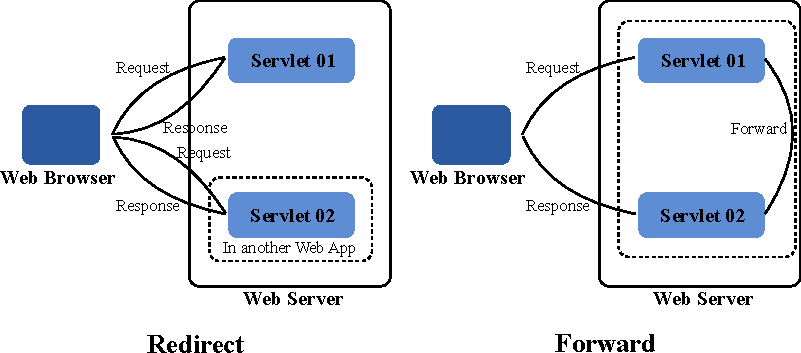
\includegraphics[width=0.8\textwidth]{images/JavaEE-ServletContext-and-Web-configuration/fig-redirect-and-forward.pdf}
\caption{重定向和转发的区别}
\label{fig:redirect-and-forword}
\end{figure}


\begin{enumerate}
\item {\hei 发生的地点不同} {\kai 重定向由客户端完成,而转发由服务器
    完成。}
\item {\hei 请求/响应的次数不同} {\kai 重定向两次请求,创建两个请求对
    象和响应对象,而转发是一次请求,只创建一个请求对象和响应对象。重
    定向无法共享请求/响应对象,而转发可以。}
\item {\hei 目标位置不同} {\kai 重定向可以跳转到Web应用以外的文档,而
    转发只能在一个Web内部文件中间进行。}
\end{enumerate}

\notice{注意}

转发之前不应有响应发送,否则导致异
常javax.servlet.IllegalStateException抛出。

